 \section{Theorie}
\label{sec:Theorie}

Ein Stoff kann in verschiedenen Phasen vorliegen. Dies sind insbesondere die Aggregatzustände fest, flüssig und gasförmig.
Der Übergang von einer Phase in die andere hängt von der Temperatur $T$ und dem Druck $p$ ab.

\begin{figure}
  \centering
  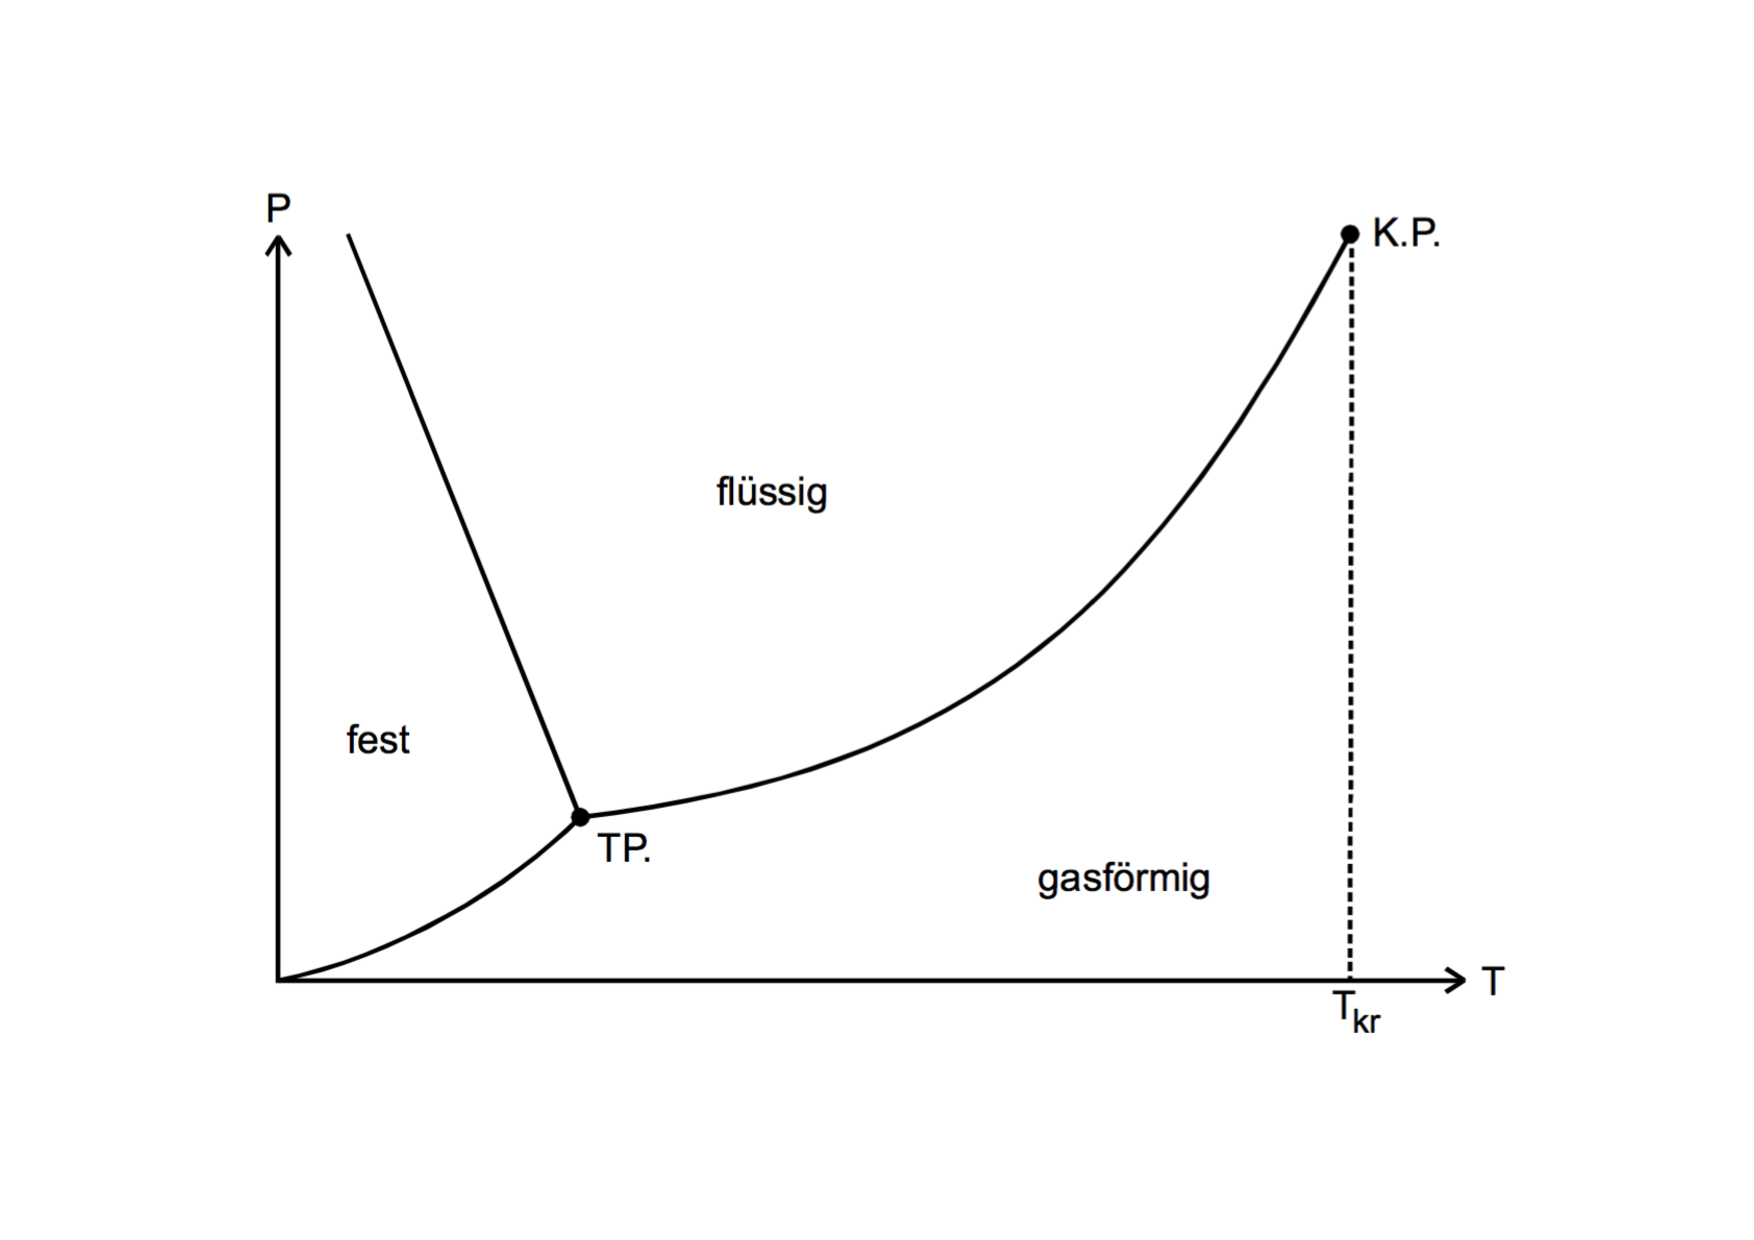
\includegraphics[height = 8cm]{Phasendiagramm.pdf}
  \caption{Qualitatives Zustandsdiagramm des Wassers.}
  \label{fig: Wasserdiagramm}
\end{figure}

In Abbildung \ref{fig: Wasserdiagramm} ist der Druck gegen die Temperatur aufgetragen.
Hier erkennt man, dass Kurven und auch Punkte existieren in deren unmittelbarer Umgebung zwei oder auch drei(beim Punkt TP) Phasen koexistieren können.

Im Folgenden wollen wir die Dampfdruckkurve untersuchen. Sie wird von den, in Abbildung \ref{fig: Wasserdiagramm} erkennbaren Punkten TP und KP
begrenzt. In ihrer Nähe tritt das Wasser in zwei Phasen auf: Flüssig und Gasförmig. Außerdem ist auf der $p(T)$-Kurve nur ein Freiheitsgrad
vorhanden, da zu jeder Temperatur ein Druck zugeordnet ist und andersherum.

Damit eine Gas-Phase entstehen kann, müssen zunächst einige Wassermoleküle aus der flüssigen Phase austreten. Hierfür benötigen sie zusätzliche
kinetische Energie. Wir führen den Begriff der Verdampfungswärme L ein. Sie bestimmt größtenteils alleine den Verlauf der Dampfdruckkurve. L ist
strenggenommen Temperaturabhängig, wie wir in Kapitel \ref{sec: MmA2} noch sehen werden. In einer großen Spanne aber ist die Verdampfungswärme
fast konstant.

Wenn wir sie darauf beziehen, wie viel Energie ein Mol Wasser für den Phasenübergang von Flüssig zu Gasförmig benötigt ohne seine Temperatur zu
erhöhen, kommen wir auf den Begriff der molaren Verdampfungswärme $L_{m}$.

Bei Erhöhung der Temperatur erhalten die Wassermoleküle im System zusätzliche Energie und können in die Gas-Phase übertreten. Je mehr Wassermoleküle
in dieser Form vorliegen, desto höher steigt der Druck.
\newpage
